\documentclass[conference]{IEEEtran}
% \usepackage[utf8]{inputenc}
% \usepackage[T1]{fontenc}

% include packages
\usepackage{fontspec} % enable us to set different fonts
\usepackage{xeCJK}    % separate Chinese, and English settings

\usepackage{fixmath}
\usepackage{graphicx} % adding images
\usepackage{parskip}  % Paragraphs and newlines
\usepackage{listings} % syntax highlight
\usepackage{color}    %

% setting fonts
\setmainfont{Times New Roman} 
\setsansfont{Droid Sans}      
\setmonofont{Courier New}     

% \setCJKmainfont{cwTeXMing}     % 明體
% \setCJKmainfont{cwTeXYen}      % 圓體
\setCJKmainfont{cwTeXKai}      % 楷體
% \setCJKmainfont{cwTeXFangSong} % 仿宋體
% \setCJKsansfont{cwTeXKai}
% \setCJKmonofont{WenQuanYi Micro Hei Mono}

\usepackage{amssymb}
\usepackage{amsmath} % American Mathematical Society
\usepackage{mathtools}
\usepackage{algorithm}
\usepackage{algpseudocode}
\usepackage{graphics}
\usepackage{epsfig}
%\usepackage{subcaption}
\usepackage{subfigure}
\usepackage{soul,xcolor}
\usepackage{amsfonts}
\usepackage{graphicx}
\usepackage{multirow}
\usepackage{textcomp}	
\usepackage{color}
%\usepackage{ulem}
\renewcommand{\algorithmicrequire}{\textbf{Initialization:}}
\renewcommand{\algorithmicensure}{\textbf{Output:}}
\newtheorem{theorem}{Theorem}
\newtheorem{definition}{Definition}
\newtheorem{lemma}{Lemma}
\newtheorem{prop}{Proposition}
\newtheorem{proof}{Proof}
\newtheorem{remark}{Remark}
\newtheorem{assumption}{Assumption}
\hyphenation{op-tical net-works semi-conduc-tor}
\newcounter{MYtempeqncnt}
\newcommand{\ron}[1]{{\bf (Ron: #1)}}
\newcommand{\JY}[1]{{\color{blue} #1}}
\DeclarePairedDelimiter\floor{\lfloor}{\rfloor}
\DeclareMathOperator*{\argmin}{arg\,min}
\DeclareMathOperator*{\argmax}{arg\,max}
\setlength{\columnsep}{0.23 in}
\IEEEoverridecommandlockouts



\begin{document}
    \title{ % ASP Group 6 Term Project Paper Report: \\ 
    A brief comparison between Affine Projection Algorithm and Normalized Least Mean Squares Algorithm on adaptive channel equalizer designs}
    \author{\IEEEauthorblockN{110064511 陳冠銘, 110064533 陳劭珩, 110064535 陳逸衍, 110064544 楊哲寬}
    }
    \maketitle
    \begin{abstract}
        利用仿射投影演算法(Affine Projection Algorithm) 於適應性等化器設計
        以消除通道雜訊之應用。APA跟其他適應性濾波器演算法,如LMS, NLMS, RLS...相比,
        最大的優點在於能夠快速地收斂至最佳解,因此在對於需要快速得到最佳解的例子,是非常的有效。
    \end{abstract}
    \begin{IEEEkeywords}
        LMS, NLMS, Affine projection algorithm, adaptive filter, adaptive equalizer. 
    \end{IEEEkeywords}
    \IEEEpeerreviewmaketitle
    
    \section{Introduction}\label{sec_intro}
    適應性濾波器演算法中最廣為人知的方法為LMS \cite{widrow1960adaptive}是一種基於LMMSE以及梯度下降機制所設計的濾波器,其最主要關鍵的設計就是利用瞬間錯誤來得到更新方程式,然而LMS有一個很大的缺點,就是存在非均勻收斂的現象。為了能夠更進一步改善上述問題,NLMS而後被提出來 \cite{Hsia1983convergence},而NLMS僅是對更新方程式做些微改變,就能夠有效彌補LMS的缺點,因此NLMS也是一個被廣為使用的演算法。
    雖然NLMS可以有效解決非均勻收斂問題,但是NLMS與LMS同樣遇到一個應用上的困難,即當設定越小的步距參數,LMS與NLMS演算法收斂速度會越慢,對於應用在需要小步距去解決的複雜問題來說,不是個很好的選擇,因此 \cite{Ozeki1984An}\cite{Ozeki2016Theory}提出一個基於仿射投影所設計的演算法(Affine projection algorithm, 簡稱為APA),而APA最大的特點在於它可以在複雜問題中更快收斂,更適合應用在一些有需要快速收斂需求的複雜問題上。
    %%%%%%%%%%%%%%%%%%%%%%%%%%%%%%%%%%%%%%%%%%%%%%%%%
    \begin{figure}[hb]
        \centering
        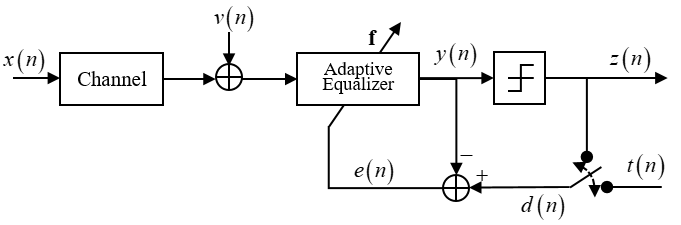
\includegraphics[width={0.9\linewidth}]{Figure/system_model.png}
        \caption{等化器方塊圖}
        \label{fig:等化器方塊圖}
        \vspace{-0.25cm}
    \end{figure}
    %%%%%%%%%%%%%%%%%%%%%%%%%%%%%%%%%%%%%%%%%%%%%%%%%
    
    此次的報告是基於APA所設計的演算法來設計適應性等化器,詳細的步驟如Fig.\ref{fig:等化器方塊圖}所示。等化器在通訊系統中是為了要來補償 ,因為 受到了通道以及雜訊 的影響,因此為了要復原傳送的信號  ,我們可以先傳送一段接收端已知的信號,叫做訓練序列  ,當訓練序列傳送時會受到環境影響,而到接收端時,因為是一段已知的信號,因此接收端可以經過一個適應性濾波器將信號做補償,盡可能的除去通道的影響而還原回原始信號。而圖中的濾波器係數為 、經過偵測後的信號為 。因此此次報告是要用APA之適應性等化器來將信號還原,另外也使用了NLMS以及APA-SE來比較性能。
    
    接下來將會依照下列區塊介紹: section \ref{sec_alog}為APA演算法說明及推導,
    section \ref{sec_sim}為各等化器設計的模擬結果,section \ref{sec_con}為結論及工作分配。
    
    \section{Algorithm}\label{sec_alog}
    
    在演算法的部分,第一部分解釋為何APA可以比NLMS還要更快收斂;第二部分則是使用基於最佳化理論的方式來證明出APA的更新方程式;第三部分則是證明APA的收斂行為。而在以下演算法中,符號$(\cdot)^T$代表轉置矩陣,$\Pi$為仿射子空間、$P_{\Pi}$代表仿射投影到$\Pi$。
    
    \subsection{空間迭代收斂證明}
    
    要如何證明在相同的迭代次數下,NLMS濾波器係數與收斂的結果相差一定會大於APA濾波器係數與收斂的結果,也就是
    \begin{align}\label{eq:1}
        \parallel \textbf{f}^o-\textbf{f}^{\left( 1 \right)}_{n+1} \parallel \geq \parallel \textbf{f}^o-\textbf{f}^{\left( 2 \right)}_{n+1} \parallel 
    \end{align}
    如Fig.\ref{fig:2a}所示,假設濾波器最佳解$\textbf{f}^o$剛好在平面$\Pi_{n-1}$及$\Pi_{n}$的交界處。其中新的濾波器係數$\textbf{f}_{n+1}$在NLMS中表示為$\textbf{f}^{\left( 1 \right)}_{n+1}$,在APA中為$\textbf{f}^o-\textbf{f}^{\left( 2 \right)}_{n+1}$,且$0<\alpha<2$,NLMS是直接垂直投影到平面$\Pi_{n}$,而APA則是投影到平面$\Pi_{n-1}$及$\Pi_{n}$。因為$P_{\Pi_{n}}\textbf{f}_n-\textbf{f}_n$與仿射子空間$\Pi_{n}$,$P_{\Pi_{n}}\textbf{f}_n-\textbf{f}_n$與$\Pi_{n} \cap \Pi_{n-1}$正交。$P_{\Pi_{n} \cap \Pi_{n-1}}\textbf{f}_n-\textbf{f}_n$與$\Pi_{n} \cap \Pi_{n-1}$也會正交。藉由這些關係,可以得到
    \begin{align}\label{eq:2}
        P_{\Pi_{n} \cap \Pi_{n-1}}\textbf{f}_n-P_{\Pi_{n}}\textbf{f}_n=P_{\Pi_{n} \cap \Pi_{n-1}}\textbf{f}_n-\textbf{f}_n-\left( P_{\Pi_{n}}\textbf{f}_n-\textbf{f}_n \right)
    \end{align}
    而\eqref{eq:2}會與$\Pi_{n} \cap \Pi_{n-1}$正交,因此,向量$P_{\Pi_{n} \cap \Pi_{n-1}}\textbf{f}_n-P_{\Pi_{n}}\textbf{f}_n$會與$P_{\Pi_{n} \cap \Pi_{n-1}}\textbf{f}_n-\textbf{f}^o$正交,依照此關係,可得
    \begin{align}\label{eq:3}
        \parallel P_{\Pi_n}\textbf{f}_n-\textbf{f}^o \parallel  \geq \parallel P_{\Pi_n \cap \Pi_{n-1}}\textbf{f}_n-\textbf{f}^o \parallel
    \end{align}
    再來假設
    \begin{align}\label{eq:4}
        &a=\parallel \textbf{f}^o-\textbf{f}_n \parallel,  b=\parallel \textbf{f}^o-P_{\Pi_{n}}\textbf{f}_n\parallel \notag \\
        &c=\parallel \textbf{f}^o-P_{\Pi_n \cap \Pi_{n-1}}\textbf{f}_n \parallel, d=\parallel \textbf{f}_n-P_{\Pi_{n}}\textbf{f}_n\parallel \notag \\
        &e=\parallel \textbf{f}_n-P_{\Pi_n \cap \Pi_{n-1}}\textbf{f}_n \parallel
    \end{align}
    如Fig. \ref{fig:2b}所示。而在Fig. \ref{fig:2b}中可以看到$\textbf{f}^o$與$\textbf{f}^{\left( 1 \right)}_{n+1}$跟$\textbf{f}^o$與$\textbf{f}^{\left( 2 \right)}_{n+1}$的距離可以藉由直角三角關係是得到,如下
    \begin{align}\label{eq:5}
        \parallel \textbf{f}^o-\textbf{f}^{\left( 1 \right)}_{n+1} \parallel^2&=b^2+\parallel \textbf{f}^{\left( 1 \right)}_{n+1}-P_{\Pi_{n}}\textbf{f}_n\parallel^2 \notag \\
        &=b^2+\left( 1-\alpha \right)^2d^2 \notag \\
        &=b^2+\left( 1-\alpha \right)^2\left( a^2-b^2 \right) \notag \\
        &=\alpha \left( 2-\alpha \right)b^2+\left( 1-\alpha \right)a^2
    \end{align}
    同樣
    \begin{align}\label{eq:6}
        \parallel \textbf{f}^o-\textbf{f}^{\left( 2 \right)}_{n+1} \parallel^2&=c^2+\parallel \textbf{f}^{\left( 2 \right)}_{n+1}-P_{\Pi_n \cap \Pi_{n-1}}\textbf{f}_n\parallel^2 \notag \\
        &=c^2+\left( 1-\alpha \right)^2e^2 \notag \\
        &=c^2+\left( 1-\alpha \right)^2\left( a^2-c^2 \right) \notag \\
        &=\alpha \left( 2-\alpha \right)c^2+\left( 1-\alpha \right)a^2
    \end{align}  
    然後$b>c$、$\alpha\left( 2-\alpha \right) \ge 0$ 將\eqref{eq:5}與\eqref{eq:6}組合,可以得到
    \begin{align}\label{eq:7}
        \parallel \textbf{f}^o-\textbf{f}^{\left( 1 \right)}_{n+1} \parallel-\parallel \textbf{f}^o-\textbf{f}^{\left( 2 \right)}_{n+1} \parallel=\alpha \left( 2-\alpha \right)\left( b^2-c^2 \right)
    \end{align}
    因為兩者相減所剩下的值恆大於等於零,因此可以得到
    \begin{align}\label{eq:8}
        \parallel \textbf{f}^o-\textbf{f}^{\left( 1 \right)}_{n+1} \parallel \geq \parallel \textbf{f}^o-\textbf{f}^{\left( 2 \right)}_{n+1} \parallel
    \end{align}
    所以證明了APA會比NLMS還要快收斂。
    %%%%%%%%%%%%%%%%%%%%%%%%%%%%%%%%%%%%%%%%%%%%%%%%%
    \begin{figure}[h]
        \centering
        \subfigure[]{
        \centering
        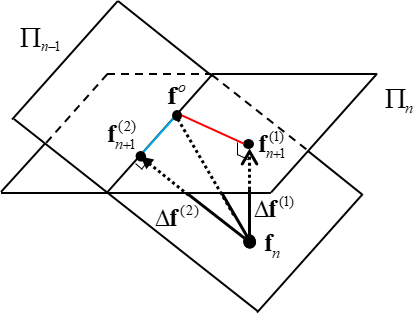
\includegraphics[width={.4\linewidth}]{Figure/fig2.png}
        \label{fig:2a}
        }
        \subfigure[]{
        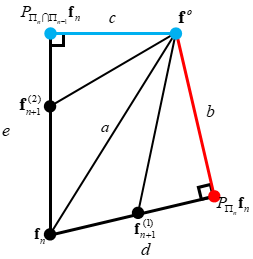
\includegraphics[width={.4\linewidth}]{Figure/fig3.png}
        \label{fig:2b}     
        }
        \caption{(a) 收斂投影圖 (b) 收斂平面圖}
    \end{figure}
    %%%%%%%%%%%%%%%%%%%%%%%%%%%%%%%%%%%%%%%%%%%%%%%%%
    %%%%%%%%%%%%%%%%%%%%%%%%%%%%%%%%%%%%%%%%%%%%%%%%%
    \begin{figure}[t]
        \centering
        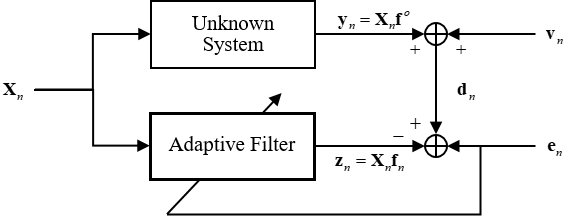
\includegraphics[width={1\linewidth}]{Figure/fig4.png}
        \caption{收斂平面圖}
        \label{fig:3}
        \vspace{-0.25cm}
    \end{figure}
    %%%%%%%%%%%%%%%%%%%%%%%%%%%%%%%%%%%%%%%%%%%%%%%%%
    \subsection{由最佳化理論證明APA的更新方程式}
    一般證明更新方程式的方式有很多種,為了能夠看出NLMS以及APA的相似之處,在此使用最佳化理論\cite{Haykin2014adaptive}來證明NLMS以及APA,而NLMS的方式如下
    \begin{align}
        & \hspace{-0.25cm} \min_{\textbf{f}} 
        & & \hspace{-1.8cm} \parallel \textbf{f}-\textbf{f}_n \parallel^2 \label{eq:9} \\ 
        & \text{s.t.} & & \hspace{-1.8cm} d \left( n \right)-\textbf{x}^T_n\textbf{f}=0 \label{eq:10}
    \end{align}
    其中式\eqref{eq:9}及\eqref{eq:10}代表的是要讓實際濾波器係數與估計的濾波器係數相差越小越好,而且要在錯誤為零的條件下達到,接著使用拉格朗日乘數可以得到NLMS的更新方程式,為
    \begin{align}\label{eq:11}
        \textbf{f}_{n+1}=\textbf{f}_{n}+\alpha e\left( n \right)\frac{\textbf{x}_n}{c+\textbf{x}^T_n\textbf{x}_n}
    \end{align}
    其中$c$為非常小的正實數。其中
    \begin{align}
        &\textbf{x}_n=
        \begin{bmatrix}
            x\left( n \right), x\left( n-1 \right), \ldots, x\left( n-M+1 \right)
        \end{bmatrix}^T\label{eq:12}\\
        &\textbf{f}_n=
        \begin{bmatrix}
            f\left( n \right), f\left( n-1 \right), \ldots, f\left( n-M+1 \right)
        \end{bmatrix}^T\label{eq:13}
    \end{align}
    $M$代表濾波器長度。
    
    而APA的證明與NLMS極為相似,差在限制除了限制當下時間點的誤差外,也考慮了$L-1$個時間點的誤差,如下所示
    \begin{align}
        & \hspace{-0.25cm} \min_{\textbf{f}} 
        & & \hspace{-1.8cm} \parallel \textbf{f}-\textbf{f}_n \parallel^2 \label{eq:14} \\ 
        & \text{s.t.} & & \hspace{-1.8cm} d \left( n \right)-\textbf{x}^T_n\textbf{f}=0 \notag \\
        &&& \hspace{-1.8cm} d \left( n-1 \right)-\textbf{x}^T_{n-1}\textbf{f}=0 \notag \\
        &&&  \vdots \notag \\
        &&& \hspace{-1.8cm} d \left( n-L+1 \right)-\textbf{x}^T_{n-L+1}\textbf{f}=0\label{eq:15}
    \end{align}
    $L$代表投影誤差長度。利用拉格朗日乘數,可以得到
    \begin{align}\label{eq:16}
        \mathcal{L}\left( \textbf{f}, \lambda_0,  \lambda_1, \ldots, \lambda_{L-1} \right)&=\parallel \textbf{f}-\textbf{f}_n \parallel^2\notag \\
        &+\sum \limits^{L-1}_{i=0}\lambda_i\left[ d\left( n-i \right)-\textbf{x}^T_{n-i}\textbf{f} \right]
    \end{align}
    並對\eqref{eq:16}中$\textbf{f}$ 偏微分令其等於零得到
    \begin{align}\label{eq:17}
        2\textbf{f}-2\textbf{f}_n-\sum \limits^{L-1}_{i=0}\lambda_i \textbf{x}_{n-i}=0 
    \end{align}
    整理得
    \begin{align}\label{eq:18}
        \textbf{f}&=\textbf{f}_n+\sum \limits^{L-1}_{i=0} \frac{\lambda_i}{2} \textbf{x}_{n-i} \notag \\
        &=\textbf{f}_n+\textbf{X}^T_n\boldsymbol{\lambda}
    \end{align}
    其中,
    \begin{align}
        &\textbf{X}_n=
        \begin{bmatrix}
            \textbf{x}_n, \textbf{x}_{n-1}, \ldots, \textbf{x}_{n-L+1}
        \end{bmatrix}^T\label{eq:19}\\
        &\boldsymbol{\lambda}=
        \begin{bmatrix}
            \frac{\lambda_0}{2}, \frac{\lambda_1}{2},\ldots, \frac{\lambda_{L-1}}{2}
        \end{bmatrix}^T\label{eq:20}
    \end{align}
    並對\eqref{eq:18}等號兩邊的左邊乘上$\textbf{X}_n$,若假設\eqref{eq:19}每列為線性獨立,且$\textbf{X}_n\textbf{X}^T_n$為非奇異矩陣,可以得到
    \begin{align}\label{eq:21}
        &\textbf{X}_n\textbf{X}^T_n\boldsymbol{\lambda}=\textbf{e}_n \notag \\
        &\boldsymbol{\lambda}=\left( \textbf{X}_n\textbf{X}^T_n \right)^{-1} \textbf{e}_n
    \end{align}
    將\eqref{eq:21}帶入\eqref{eq:18}中,可得
    \begin{align}\label{eq:22}
        &\textbf{f}=\textbf{f}_n+\textbf{X}^T_n\left( \textbf{X}_n\textbf{X}^T_n \right)^{-1} \textbf{e}_n \notag \\
        &\textbf{e}_n=\textbf{d}_n-\textbf{X}_n\textbf{f}_n
    \end{align}
    其中
    \begin{align}\label{eq:23}
        &\textbf{d}_n=
        \begin{bmatrix}
            d\left( n \right), d\left( n-1 \right), \ldots, d\left( n-L+1 \right)
        \end{bmatrix}^T
    \end{align}
    
    %%%%%%%%%%%%%%%%%%%%%%%%%%%%%%%%%%%%%%%%%%%%%%%%%
    \begin{figure*}[t]
        \subfigure[]{
        \centering
        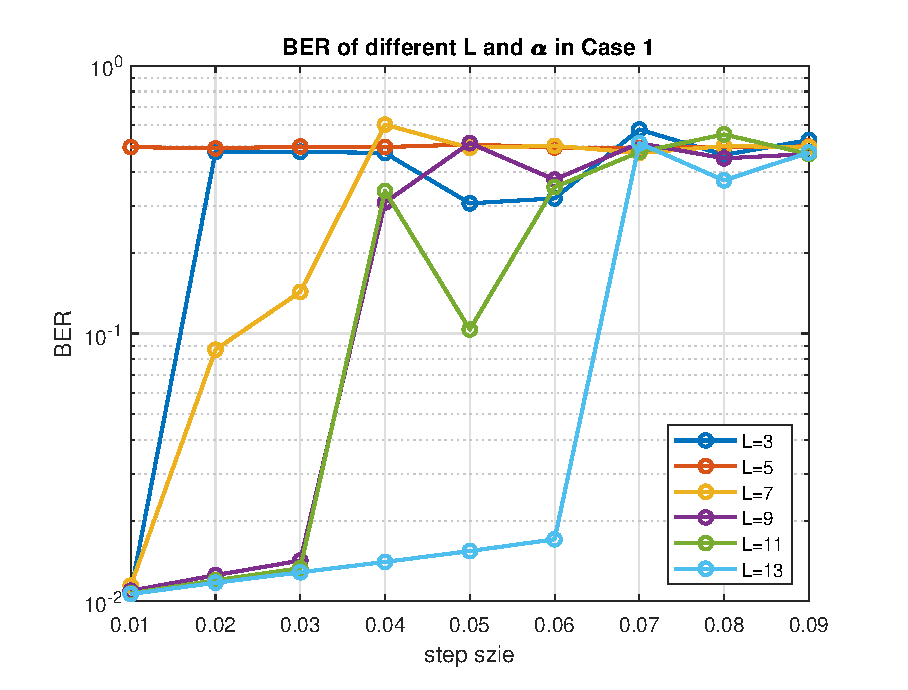
\includegraphics[width={.3\linewidth}]{Figure/APA1.eps}
        \label{fig:4a}
        }
        \subfigure[]{
        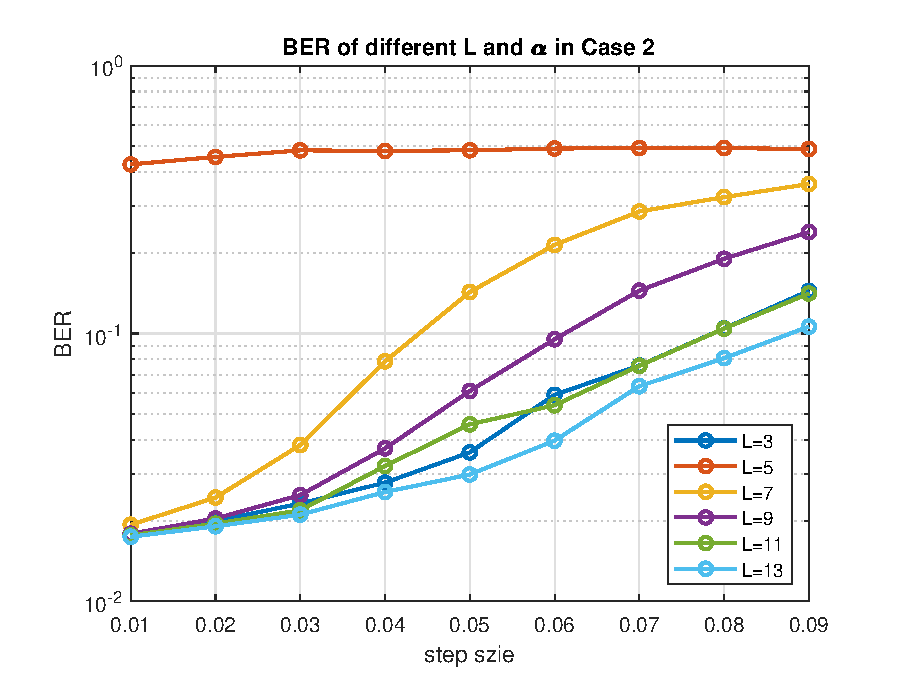
\includegraphics[width={.3\linewidth}]{Figure/APA2.eps}
        \label{fig:4b}     
        }
        \subfigure[]{
        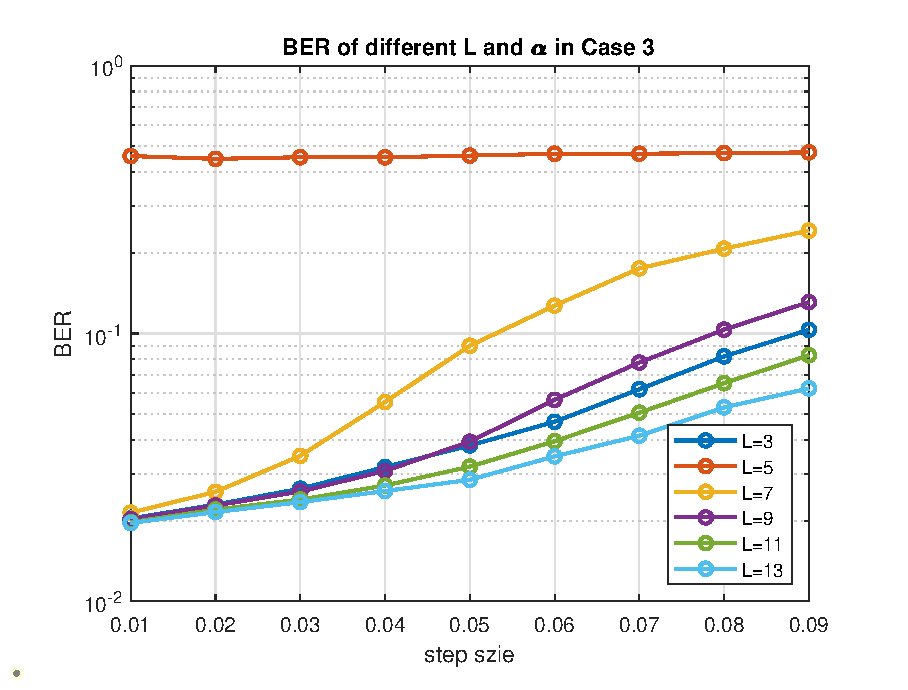
\includegraphics[width={.3\linewidth}]{Figure/APA3.eps}
        \label{fig:4c}          
        }
        \subfigure[]{
        \centering
        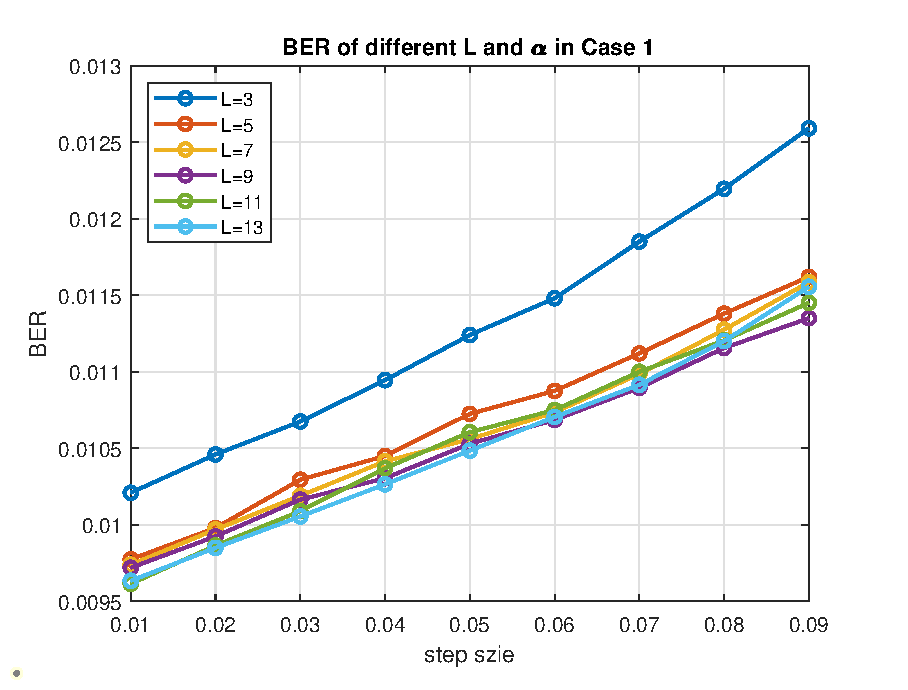
\includegraphics[width={.3\linewidth}]{Figure/NLMS1.eps}
        \label{fig:4d}
        }
        \subfigure[]{
        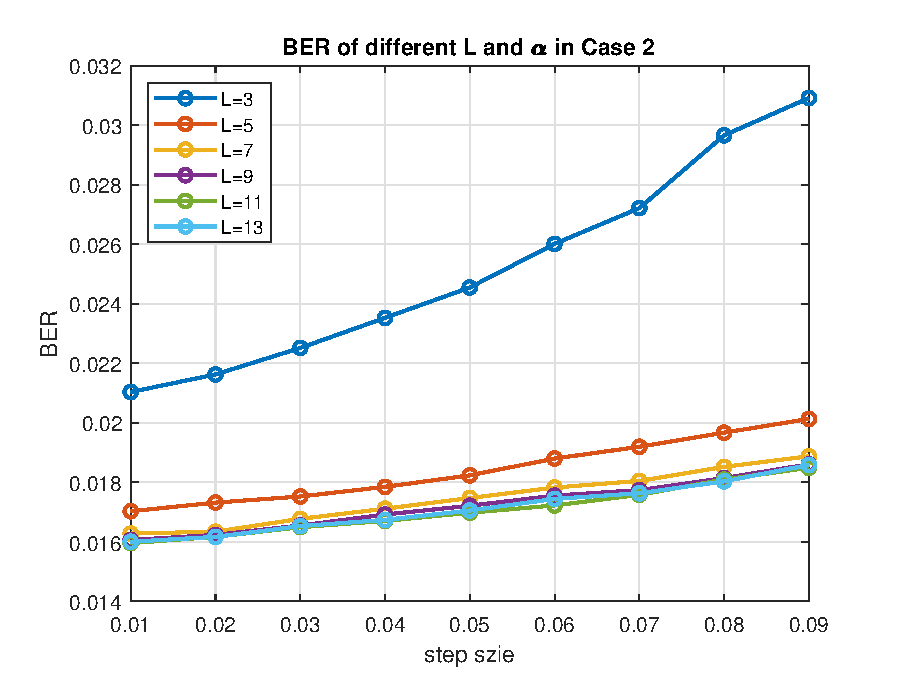
\includegraphics[width={.3\linewidth}]{Figure/NLMS2.eps}
        \label{fig:4e}     
        }
        \subfigure[]{
        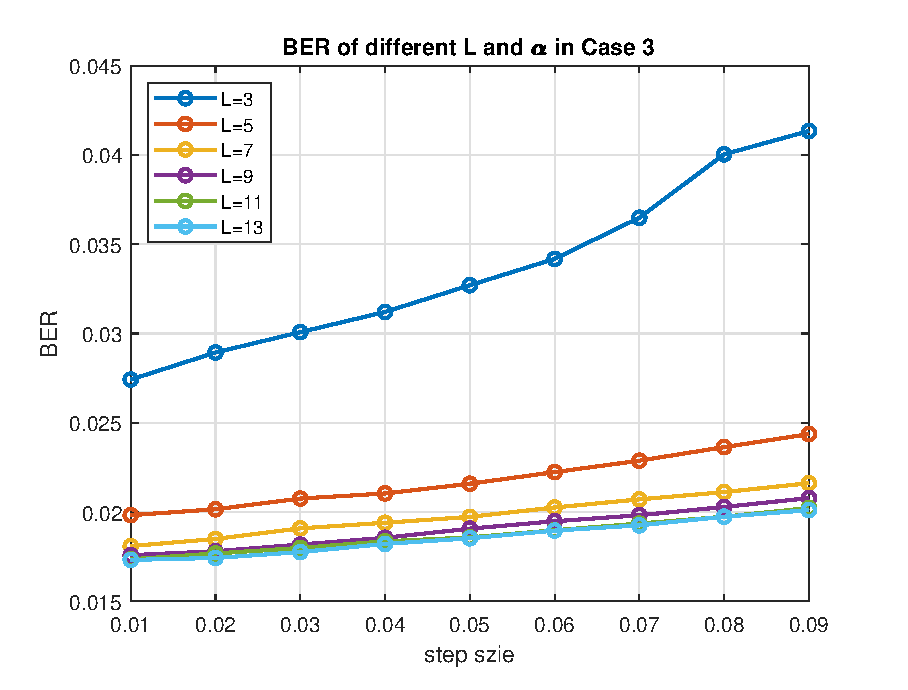
\includegraphics[width={.3\linewidth}]{Figure/NLMS3.eps}
        \label{fig:4f}          
        }
        \caption{(a) APA在static channel的BER 
                 (b) APA在quasi-static channel的BER 
                 (c) APA在time varying channel的BER 
                 (d) NLMS在static channel的BER 
                 (e) NLMS在quasi-static channel的BER 
                 (f) NLMS在time varying channel的BER}
    \end{figure*}
    %%%%%%%%%%%%%%%%%%%%%%%%%%%%%%%%%%%%%%%%%%%%%%%%%
    
    因此APA的更新方程式為
    \begin{align}\label{eq:24}
        \textbf{f}_{n+1}&=\textbf{f}_n+\alpha \textbf{X}^T_n\left( \textbf{X}_n\textbf{X}^T_n \right)^{-1} \textbf{e}_n \notag \\
        &=\textbf{f}_n+\alpha \textbf{X}^{\dag}_n\textbf{e}_n
    \end{align}
    其中$\left( \cdot \right)^{\dag}$代表虛擬反矩陣。再來,為了簡化更新方程式,我們將$\textbf{e}_n$取sign,得到新的更新方程式為
    \begin{align}\label{eq:25}
         \textbf{f}_{n+1}=\textbf{f}_n+\alpha \textbf{X}^T_n\left( \textbf{X}_n\textbf{X}^T_n \right)^{-1} sgn \left( \textbf{e}_n \right)
    \end{align}
    \subsection{APA收斂行為}
    要證明收斂行為,我們先假設是一個系統識別的問題,Fig. \ref{fig:3}所示。
    
    其中,輸入信號$\textbf{X}_n$為廣義穩態信號、$\textbf{v}_n$為AWGN、且$\textbf{X}_n$與$\textbf{v}_n$相互獨立。未知系統中的係數為$\textbf{f}^o$,更新方程式如下
    \begin{align}\label{eq:26}
        & \textbf{f}_{n+1} = \textbf{f}_{n} + \alpha\textbf{X}_{n}^T{\left(\textbf{X}_{n} \textbf{X}_{n}^T\right)}^{-1}\textbf{e}_{n} \notag \\
        & = \textbf{f}_{n} + \alpha\textbf{X}_{n}^T{\left(\textbf{X}_{n} \textbf{X}_{n}^T\right)}^{-1}\left(\textbf{d}_{n} - \textbf{X}_{n}\textbf{f}_{n} \right)
    \end{align}
    而$\textbf{d}_{n} = \textbf{X}_{n}^T\textbf{f}_{n}^{o} + \textbf{v}_{n}$,帶回\eqref{eq:26}式如下
    \begin{align}\label{eq:27}
        & \textbf{f}_{n+1} = \textbf{f}_{n} + \alpha\textbf{X}_{n}^T{\left(\textbf{X}_{n} \textbf{X}_{n}^T\right)}^{-1}\left(\textbf{X}_{n}^T\textbf{f}_{n}^{o} + \textbf{v}_{n} - \textbf{X}_{n}\textbf{f}_{n}  \right)
    \end{align}
    將\eqref{eq:27}簡化可得
    \begin{align}\label{eq:28}
        & \widetilde{\textbf{f}}_{n+1} = \left(\textbf{I} - \alpha\textbf{X}_{n}^T{\left(\textbf{X}_{n} \textbf{X}_{n}^T\right)}^{-1}\textbf{X}_{n} \right) \widetilde{\textbf{f}}_{n} \notag \\
        & - \alpha\textbf{X}_{n}^T{\left(\textbf{X}_{n} \textbf{X}_{n}^T\right)}^{-1}\textbf{v}_{n}
    \end{align}
    \eqref{eq:28}中第二項因為$\textbf{X}_n$與$\textbf{v}_n$相互獨立因此可以直接省略,此外$\widetilde{\textbf{f}}_{n+1} = \textbf{f}_{o} - \textbf{f}_{n}$。
    
    假設$\textbf{A}_{n} = \textbf{X}_{n}^T{\left(\textbf{X}_{n} \textbf{X}_{n}^T\right)}^{-1}\textbf{X}_{n}$,
    而藉由 \eqref{eq:28}可以證明在$0 < \alpha < 2$的條件下,$\widetilde{\textbf{f}}$將會收斂到0。首先,將 \eqref{eq:28}兩邊同
    取期望值,並且做化簡可得
    \begin{align}\label{eq:29}
        E \{ \widetilde{\textbf{f}}_{n+1} \} = \left( \textbf{I} - \alpha E \{\left( \textbf{A}_{n} \right)\}\right) E \{\widetilde{\textbf{f}}_{n}\}
    \end{align}
    再來將$E \{ \textbf{A}_{n} \}$做特徵分解如下
    \begin{align}\label{eq:30}
        E \{ \widetilde{\textbf{f}}_{n+1} \} = \left( \textbf{I} - \alpha \textbf{Q} \boldsymbol{\Lambda} \textbf{Q}^{T}\right) E\{ \widetilde{\textbf{f}}_{n}\}
    \end{align}
    \eqref{eq:30}中的$\textbf{Q}$為特徵向量,其對應到的特徵值為$\boldsymbol{\Lambda} = {diag}\left( {\lambda}_{1}, {\lambda}_{2}, \ldots, {\lambda}_{k}\right)$,再來假設$\widehat{\textbf{f}}_{n} = \textbf{Q}^{T}E\{\widetilde{\textbf{f}}_{n} \}$帶回上式,會得到
    \begin{align}\label{eq:31}
        \textbf{Q}^T E\{ \widetilde{\textbf{f}}_{n+1} \}=\textbf{Q}^TE\{\widehat{\textbf{f}}_{n}\}-\alpha\textbf{Q}^T\textbf{Q}\boldsymbol{\Lambda}\textbf{Q}^TE\{ \widetilde{\textbf{f}}_{n}\}
    \end{align}
    
    \begin{align}\label{eq:32}
        \widehat{\textbf{f}}_{n+1}&=\widehat{\textbf{f}}_{n} -\alpha \boldsymbol{\Lambda}\widehat{\textbf{f}}_{n} \notag \\
        &=\left( 1-\alpha \boldsymbol{\Lambda} \right) \widehat{\textbf{f}}_{n} \notag \\
        \widehat{f}_n\left( j \right)&=\left( 1-\alpha \lambda_j \right)^n\widehat{f}_0\left( j \right)
    \end{align}
    而其中$0<\lambda_j<n$,因此當$0<\alpha<2$時,其括號內值都會小於$0$,因此可以得知$\widetilde{\textbf{f}}_n$將會收斂至$0$。
    
    \section{Simulations}\label{sec_sim}
    
    由Fig. 4所示可以看到,根據我們嘗試不同filter length L與不同step size $\alpha$的模擬結果,無論是NLMS或 是APA,選擇越高的filter length L與越小的step size $\alpha$所得到的BER會越低。由上述模擬結果推估,filter length L大約在11、13左右時效能會逐漸收斂。因此我們最後使用$L=13$。若設備與時間許可的話,理論上更高的filter length L應能達到更好的結果。
    至於最終演算法選擇,由於NLMS的效能稍微比APA更佳(即BER較低),因此在這個通道雜訊消除的問題應用上,我們會選用NLMS來完成。
    

    \section{Conclusion}\label{sec_con}
    LMS是利用瞬間的錯誤來得到更新方程式,LMS有一個很大的缺點,就是存在非均勻收斂的現象。為了能夠更進一步改善上述問題,NLMS而後被提出來,雖然NLMS可以有效解決非均勻收斂問題,但是NLMS與LMS同樣遇到一個應用上的困難,即當設定越小的步距參數,LMS與NLMS演算法收斂速度會越慢,對於應用在需要小步距去解決的複雜問題來說,不是個很好的選擇,因此利用仿射投影演算法(Affine projection algorithm)去優化,而APA最大的優點在於它可以在 複雜問題中更快收斂,更適合應用在一些有需要快速收斂需求的複雜問題上。
    
    我們這次對NLMS與APA這兩種演算法進行簡單的分析與比較。APA的優勢在於收斂速度較快,不過它的演算法複雜度也較高。因此,需要考量問題需求及硬體資源、時間成本等因素,來判斷選擇何種演算法更合適。如果愈解決的問題相當複雜且有快速收斂的要求,APA可能是合適的選擇;而如果當BER比收斂速度更加重要時,則是NLMS比APA更加合適。從模擬結果來看,雖然APA收斂速度快,但相比之下其BER表現相較NLMS在簡單的雜訊消除問題下並沒有顯著的優勢,故APA在等化器演算法設計中並不是最佳解,但若只看MSE,因為APA收斂速度快的緣故,是較NLMS更佳的演算法。
    
    最後是工作分配,本組同學都積極參與期末專案實作,雖然投入時間不同但大家整體貢獻都差不多,謝謝老師及助教學長。
    \begin{table}[!ht]
    \centering
        \begin{tabular}{|| c | c | c | c ||} 
            \hline\hline
            學號 & 姓名 & 工作內容 &  貢獻度 \\ [1ex]
            \hline\hline
            110064511 & 陳冠銘 & APA演算法數學推導, 及物理意義分析 & 25\% \\ [1ex]
            \hline
            110064533 & 陳劭珩 & Latex撰寫, 上台報告, 演算法程式實作  & 25\%  \\ [1ex]
            \hline
            110064535 & 陳逸衍 & NLMS程式實作, 圖表, 及投影片製作 & 25\%  \\ [1ex]
            \hline
            110064544 & 楊哲寬 & RLS程式實作, 資料蒐集, 及程式除錯 & 25\% \\ [1ex]
            \hline\hline
        \end{tabular}
        \label{table} \caption{ASP Term Project 第6組工作分配表}
    \end{table}
    
    
    \bibliographystyle{IEEEtran} 
    \bibliography{IEEEabrv,reference}
\end{document}
